\documentclass[10pt,a4paper,onecolumn]{article}
% \usepackage[utf8]{inputenc}
\usepackage{marginnote}
\usepackage{graphicx}
\usepackage{xcolor}
\usepackage{authblk,etoolbox}
\usepackage{titlesec}
\usepackage{calc}
\usepackage{hyperref}
\hypersetup{breaklinks=true,
            bookmarks=true,
            pdfauthor=
{
      Tallec Corentin,
      Blier Léonard,
      Kalainathan Diviyan,
  },
            pdftitle=
{
[Re] Recurrent World Models Facilitate Policy Evolution
},
            colorlinks=true,
            citecolor=blue,
            urlcolor=blue,
            linkcolor=blue,
            pdfborder={0 0 0}}
\urlstyle{same}
\usepackage{tcolorbox}
\usepackage{ragged2e}
\usepackage{fontspec}
\usepackage{fontawesome}
\usepackage{caption}
\usepackage{listings}
\lstnewenvironment{code}{\lstset{language=Haskell,basicstyle=\small\ttfamily}}{}



%\usepackage{fancyvrb}
%\VerbatimFootnotes
%\usepackage{graphicx}
%\usepackage{mdframed}
%\newmdenv[backgroundcolor=lightgray]{Shaded}


\usepackage{longtable,booktabs}

\usepackage[
  backend=biber,
%  style=alphabetic,
%  citestyle=numeric
]{biblatex}
\bibliography{bibliography.bib}



% --- Macros ------------------------------------------------------------------
\renewcommand*{\bibfont}{\small \sffamily}

\definecolor{red}{HTML}{CF232B}
\newcommand{\ReScience}{Re{\bfseries \textcolor{red}{Science}}}

\newtcolorbox{rebox}
   {colback=blue!5!white, colframe=blue!40!white,
     boxrule=0.5pt, arc=2pt, fonttitle=\sffamily\scshape\bfseries,
     left=6pt, right=20pt, top=6pt, bottom=6pt}

\newtcolorbox{repobox}
   {colback=red, colframe=red!75!black,
     boxrule=0.5pt, arc=2pt, left=6pt, right=6pt, top=3pt, bottom=3pt}

% fix for pandoc 1.14     
\newcommand{\tightlist}{%
  \setlength{\itemsep}{1pt}\setlength{\parskip}{0pt}\setlength{\parsep}{0pt}}

% --- Style -------------------------------------------------------------------
\renewcommand*{\bibfont}{\small \sffamily}
\renewcommand{\captionfont}{\small\sffamily}
\renewcommand{\captionlabelfont}{\bfseries}

\makeatletter
\renewcommand\@biblabel[1]{{\bf #1.}}
\makeatother

% --- Page layout -------------------------------------------------------------
\usepackage[top=3.5cm, bottom=3cm, right=1.5cm, left=1.5cm,
            headheight=2.2cm, reversemp, includemp, marginparwidth=4.5cm]{geometry}

% --- Section/SubSection/SubSubSection ----------------------------------------
\titleformat{\section}
  {\normalfont\sffamily\Large\bfseries}
  {}{0pt}{}
\titleformat{\subsection}
  {\normalfont\sffamily\large\bfseries}
  {}{0pt}{}
\titleformat{\subsubsection}
  {\normalfont\sffamily\bfseries}
  {}{0pt}{}
\titleformat*{\paragraph}
  {\sffamily\normalsize}


% --- Header / Footer ---------------------------------------------------------
\usepackage{fancyhdr}
\pagestyle{fancy}
%\renewcommand{\headrulewidth}{0.50pt}
\renewcommand{\headrulewidth}{0pt}
\fancyhead[L]{\hspace{-1cm}\includegraphics[width=4.0cm]{rescience-logo.pdf}}
\fancyhead[C]{}
\fancyhead[R]{} 
\renewcommand{\footrulewidth}{0.25pt}

\fancyfoot[L]{\hypersetup{urlcolor=red}
              \sffamily \ReScience~$\vert$
              \href{http://rescience.github.io}{rescience.github.io}
              \hypersetup{urlcolor=blue}}
\fancyfoot[C]{\sffamily 1 - \thepage}
\fancyfoot[R]{\sffamily Sep 2015 $\vert$
                        Volume \textbf{1} $\vert$
                        Issue \textbf{1}}
\pagestyle{fancy}
\makeatletter
\let\ps@plain\ps@fancy
\fancyheadoffset[L]{4.5cm}
\fancyfootoffset[L]{4.5cm}

% --- Title / Authors ---------------------------------------------------------
% patch \maketitle so that it doesn't center
\patchcmd{\@maketitle}{center}{flushleft}{}{}
\patchcmd{\@maketitle}{center}{flushleft}{}{}
% patch \maketitle so that the font size for the title is normal
\patchcmd{\@maketitle}{\LARGE}{\LARGE\sffamily}{}{}
% patch the patch by authblk so that the author block is flush left
\def\maketitle{{%
  \renewenvironment{tabular}[2][]
    {\begin{flushleft}}
    {\end{flushleft}}
  \AB@maketitle}}
\makeatletter
\renewcommand\AB@affilsepx{ \protect\Affilfont}
%\renewcommand\AB@affilnote[1]{{\bfseries #1}\hspace{2pt}}
\renewcommand\AB@affilnote[1]{{\bfseries #1}\hspace{3pt}}
\makeatother
\renewcommand\Authfont{\sffamily\bfseries}
\renewcommand\Affilfont{\sffamily\small\mdseries}
\setlength{\affilsep}{1em}

\LetLtxMacro{\OldIncludegraphics}{\includegraphics}
\renewcommand{\includegraphics}[2][]{\OldIncludegraphics[width=12cm, #1]{#2}}


% --- Document ----------------------------------------------------------------
\title{[Re] Recurrent World Models Facilitate Policy Evolution}

    \usepackage{authblk}
                        \author[†, 1]{Tallec Corentin}
                    \author[†, 1, 2]{Blier Léonard}
                    \author[1]{Kalainathan Diviyan}
                            \affil[1]{TAckling the Underspecified,
Universite Paris Sud, Orsay, France}
                    \affil[2]{Facebook Artificial Intelligence Research,
Paris}
                    \affil[†]{Equal contribution}
            
\date{\vspace{-5mm}
      \sffamily \small \href{mailto:corentin.tallec@u-psud.fr}{corentin.tallec@u-psud.fr}}


\setlength\LTleft{0pt}
\setlength\LTright{0pt}


\begin{document}
\maketitle

\marginpar{
  %\hrule
  \sffamily\small
  %\vspace{2mm}
  {\bfseries Editor}\\
  Name Surname\\

  {\bfseries Reviewers}\\
        Name Surname\\
        Name Surname\\
  
  {\bfseries Received}  Feb, 22, 2019\\
  {\bfseries Accepted}  Sep, 1, 2015\\
  {\bfseries Published} Sep, 1, 2015\\

  {\bfseries Licence}   \href{http://creativecommons.org/licenses/by/4.0/}{CC-BY}

  \begin{flushleft}
  {\bfseries Competing Interests:}\\
  The authors have declared that no competing interests exist.
  \end{flushleft}

  \hrule
  \vspace{3mm}

  \hypersetup{urlcolor=white}
  
    \vspace{-1mm}
  \begin{repobox}
    \bfseries\normalsize
      \href{http://github.com/rescience/rescience-submission/article}{\faGithubAlt~Article repository}
  \end{repobox}
      \vspace{-1mm}
  \begin{repobox}
    \bfseries\normalsize
      \href{http://github.com/rescience/rescience-submission/code}{\faGithubAlt~Code repository}
  \end{repobox}
        \hypersetup{urlcolor=blue}
}

\begin{rebox}
\sffamily {\bfseries A reference implementation of}
\small
\begin{flushleft}
\begin{itemize}
    \item[→] Recurrent World Models Facilitate Policy Evolution, David
Ha and Jürgen Schmidhuber, NeurIPS 2018 Conference
  \end{itemize}\par
\end{flushleft}
\end{rebox}


\hypertarget{introduction}{%
\section{Introduction}\label{introduction}}

Recently, Deep Reinforcement Learning (DRL) has achieved impressive
results in a variety of domains, such as video game playing
(\textcite{mnih}) zero-sum games (\textcite{silver}), and continuous
control (\textcite{ddpg}). Still, DRL approaches are often brittle,
sensitive to small changes in hyperparameters, implementation details
and minor environment perturbations. Besides, training performance can
widely vary from run to run. Those factors often make reproduction of
experimental results challenging (\textcite{henderson},
\textcite{rlblogpost}).

In addition to its sensitivity, DRL is also known to be sample
inefficient, in the sense that it requires huge amounts of environment
interactions to obtain good results, even for simple tasks. Model-based
reinforcement learning has gained interest to improve sample efficiency.
With an accurate and computationally cheap model of the world, the
burden of collecting new samples could be considerably alleviated, since
the model could, in principle, generate huge amounts of reliable
samples, and be used for planning without interacting with the
environment. Besides, features provided by a predictive model of the
world could constitue relevant inputs to a controller, and ease the
optimization process.

\textcite{NIPS2018_7512} provided a simple, yet successful model-based
reinforcement learning approach. It revolves around a three part model,
comprised of:

\begin{enumerate}
\def\labelenumi{\arabic{enumi}.}
\tightlist
\item
  A Variational Auto-Encoder (\textcite{kingma}), a generative model,
  which learns both an encoder and a decoder. The encoder's task is to
  compress the input images into a compact latent representation. The
  decoder's task is to recover the original image from the latent
  representation.
\item
  A Mixture-Density Recurrent Network (\textcite{graves}), trained to
  predict the latent encoding of the next frame given past latent
  encodings and actions. The mixture-density network outputs a Gaussian
  mixture for predicting the distribution density of the next latent
  variable.
\item
  A simple linear Controller. It takes as inputs both the latent
  encoding of the current frame and the hidden state of the MDN-RNN
  given past latents and actions and outputs an action. It is trained to
  maximize the cumulated reward using the Covariance-Matrix Adaptation
  Evolution-Strategy (\textcite{hansen}), a generic gradient-free black
  box optimization algorithm.
\end{enumerate}

\begin{figure}
\centering
\includegraphics{img/archfig.pdf}
\caption{The three parts of the architecture (from the original
paper)\label{fig:archi}}
\end{figure}

On a given environment, the model is trained sequentially as follows:

\begin{enumerate}
\def\labelenumi{\arabic{enumi}.}
\tightlist
\item
  Sample randomly generated rollouts from a well suited \emph{random
  policy}.
\item
  Train the VAE on images drawn from the rollouts.
\item
  Train the MDN-RNN on the rollouts encoded using the encoder of the
  VAE. To reduce computational load, we trained the MDN-RNN on fixed
  size subsequences of the rollouts.
\item
  Train the controller while interacting with the environment using
  CMA-ES. At each time step, the controller takes as input both the
  encoded current frame and the recurrent state of the MDN-RNN, which
  contains information about all previous frames and actions.
\end{enumerate}

Alternatively, if the MDN-RNN is good enough at modelling the
environment, the controller can be trained directly on simulated
rollouts in the dreamt environment.

\hypertarget{methods}{%
\section{Methods}\label{methods}}

\hypertarget{reproducibility-of-the-original-results}{%
\subsection{Reproducibility of the original
results}\label{reproducibility-of-the-original-results}}

We reproduced the authors results on the CarRacing environment
(\textcite{gym}). We only used the paper description, and took the same
hyperparameters as the original paper, unless stated otherwise below, or
originally unspecified. We did not use any original sources, and we did
not contact the authors. The exact training procedure is detailled
below.

\hypertarget{data-generation}{%
\subsubsection{Data generation}\label{data-generation}}

The original paper started by generating rollouts using a random policy
interacting with the environment. The policy was not specified. In our
experiments we tested two types of policies. The first policy generates
independant standard normal actions at each step. The second policy
generates actions according to a discretized brownian motion, with a
discretization parameter of \(\frac{1}{50}\). This means that each
component of the action (the action is three dimensional) is generated
as \[a^k_{t+1} = a^k_{t} + \frac{1}{\sqrt{50}} \varepsilon^k_t\] where
the \(\varepsilon\)'s are i.i.d. standard normal random variables. The
data samples generated by the first policy lack diversity, and the car
only moves in a very restricted area of the track. The samples generated
by the second policy, on the other are much more diverse, and were
consequently used for the next stages of training. The original paper
generated 10,000 rollouts. For our replication, we generated 1,000
rollouts, to reduce the computational load.

\hypertarget{variational-auto-encoder-vae-training}{%
\subsubsection{Variational auto-encoder (VAE)
training}\label{variational-auto-encoder-vae-training}}

The VAE is trained following the training procedure of the original
paper, on the rollouts previously generated. The model is the same as
the one detailled in the paper. The first \(600\) rollouts are used as a
training set, and the next \(400\) as a validation set. The VAE is
optimized using Adam (\textcite{adam}) with default hyperparameters,
learning rate \(10^{-3}\), \(\beta_1=0.9\), \(\beta_2=0.999\). Since the
dataset is quite large, validation is perfomed each time a fifth of the
dataset has been processed. Each step of validation is performed on
\(200\) samples of the validation dataset. The learning rate is halved
each time the validation performance has not improved for \(5\)
consecutive evaluations. Training is stopped when the validation
performance has not improved for \(30\) consecutive evaluations.
Training was performed on a single Quadro GP100 GPU, with 16Go of RAM.

\hypertarget{mixture-density-recurrent-neural-network-mdn-rnn-training}{%
\subsubsection{Mixture Density Recurrent Neural Network (MDN-RNN)
training}\label{mixture-density-recurrent-neural-network-mdn-rnn-training}}

Similarily the MDN-RNN is trained following the original paper
procedure. The model is the same as the one detailled in the paper. The
training splits are the same as for the VAE, and evaluations are also
performed using the same schedule. The network is trained and validated
on subrollouts of length \(32\). RMSprop (\textcite{rmsprop}) is used to
optimize the MDN-RNN, with a learning rate \(10^{-3}\), and
\(\alpha=0.9\). The learning rate schedule and early stopping policy of
the VAE training are used without any modification. Training was
performed on a single Quadro GP100 GPU, with 16Go of RAM.

\hypertarget{controller-training-with-cmaes}{%
\subsubsection{Controller training with
CMAES}\label{controller-training-with-cmaes}}

Finally, the controller is trained using the Covariance Matrix
Adaptation Evolution Strategy (\textcite{hansen}), using the python
library pycma (\textcite{pycma}). As in the original paper, the
controller is a linear network that takes as inputs the concatenation of
the output of the VAE and the hidden layer of the MDN-RNN. For a set of
parameters of the controller, the loss function is obtained by averaging
the returns from \(16\) rollouts of length at most \(1000\). The
population size used for CMAES is \(64\), and an initial standard
deviation of \(0.1\) is used. Rollouts are executed parallely, on \(64\)
threads, with models sharing \(8\) V100 GPUs.

\hypertarget{results}{%
\section{Results}\label{results}}

\hypertarget{reproducibility}{%
\subsection{Reproducibility}\label{reproducibility}}

On the CarRacing-v0 environment, results were reproducible with relative
ease. The model achieved good results on the first try, relatively to
the usual reproducibility standards of deep reinforcement learning
algorithms (\textcite{rlblogpost}, \textcite{henderson}). Our own
implementation reached a best score of 895, below the 906 reported in
the paper, but much better than the second best benchmark reported which
is around 780. Results are further detailled in the tables and
fig.~~\ref{fig:curves}. Fig. ~\ref{fig:curves} displays the learning
curves of CMAES in the three considered setups. Solid lines represent
the mean performance and standard deviation of the population, while
dashed line represent the maximal performance. At test time, we select
the best performing element of the CMAES population.

\hypertarget{additional-experiments}{%
\subsection{Additional experiments}\label{additional-experiments}}

\hypertarget{studying-the-impact-of-the-world-model}{%
\subsubsection{Studying the impact of the World
Model}\label{studying-the-impact-of-the-world-model}}

We wanted to test the impact of the MDN-RNN on the results. Indeed, we
observed during training that the model was rapidly learning the easy
part of the dynamic, but mostly failed to account for long term effects
and multimodality.

In the original paper, the authors performed an ablation study, and
compared their results with a model without the MDN-RNN. They obtained
the following scores:

\begin{longtable}[]{@{}cc@{}}
\toprule
Method & Average score\tabularnewline
\midrule
\endhead
Full World Models \textcite{NIPS2018_7512} & 906 ± 21\tabularnewline
without MDN-RNN \textcite{NIPS2018_7512} & 632 ± 251\tabularnewline
\bottomrule
\end{longtable}

Still, we wanted to investigate this question even more. We also trained
the controller, but with an untrained MDN-RNN instead of the trained one
(we kept it at its random initialization values). Similarily, we tried
training a controller with both an untrained MDN-RNN and an untrained
VAE. Surprisingly, controllers trained with untrained recurrent models
achieve results close to the values of the original controller, while
controllers with both untrained VAE and MDN-RNN achieves very low
performance.

\begin{longtable}[]{@{}cl@{}}
\toprule
Method & Average score\tabularnewline
\midrule
\endhead
With a trained MDN-RNN & 895 ± 79\tabularnewline
With an untrained MDN-RNN & 866 ± 69\tabularnewline
With untrained MDN-RNN and VAE & 131 ± 66\tabularnewline
\bottomrule
\end{longtable}

It seems that the training of the MDN-RNN does not significantly improve
the performance. Our interpretation of this phenomenon is that even if
the recurrent model is not able to predict the next state of the
environment, its recurrent state still contains some crucial information
on the environment dynamic. Without a recurrent model, first-order
information such as the velocity of the car is absent from individual
frames, and consequently from latent codes. Therefore, strategies learnt
without the MDN-RNN cannot use such information. Even a random MDN-RNN
still holds some useful temporal information, which is enough to learn a
good strategy on this problem. This may relate to observations made in
the field of \emph{echo state networks} (ESN, \textcite{jaeger-tuto}).
ESNs consist in untrained but properly initialized reservoir recurrent
networks, which, along with properly trained output weights, prove
sufficient to solve problems with non trivial temporal dependencies. In
our case, the untrained MDN-RNN seems to also behave like a reservoir
for temporal information, necessary to solve the task at hand.

\hypertarget{using-a-training-pipeline-mixing-the-different-steps}{%
\subsubsection{Using a training pipeline mixing the different
steps}\label{using-a-training-pipeline-mixing-the-different-steps}}

As stated in the original paper, the method is limited, in the sense
that the VAE and MDRNN are only trained on random rollouts at the very
beginning. They might not model properly the data distribution after the
policy is trained.

To aleviate this issue, the original paper proposed to periodically
retrain the VAE and the MDRNN after a certain number of controller
training iterations.

We complement the results of the original paper by applying this
procedure on the Car Racing environment. Every fifth iteration of
controller training, a dataset of 1000 rollouts is generated from the
current policy, and the VAE and MDRNN are retrained. Both the VAE and
MDRNN parameters are initialized to their respective parameters at the
end of the previous training cycle, and training is halted after 3 non
improving epochs.

Using this learning pipeline improves the performance of learning, both
in tern of final performance and number of controller training steps.

\begin{longtable}[]{@{}cl@{}}
\toprule
Method & Average score\tabularnewline
\midrule
\endhead
Standard training procedure & 895 ± 79\tabularnewline
Pipeline & 910 ± 52\tabularnewline
\bottomrule
\end{longtable}

Using this pipeline is expensive in term of computation and sample
efficiency, since it requires generating new rollouts between each
retraining. The sample efficiency issue could be mitigated by training
the VAE and MDRNN on rollouts generated during the controller training
steps.

Another potential limitation of this pipeline is that, after retraining,
the MDRNN and VAE might only model properly trajectories coming from the
current (better) policy. For example in the Car Racing environment, when
only faced with trajectories that remain on the road, the agent might
forget the out of road dynamic, which could deteriorate performances.
While we believe this could be problematic in complex environment, such
issues seem not to arise on the Car Racing environment.

\hypertarget{conclusion}{%
\section{Conclusion}\label{conclusion}}

We reproduced the paper ``World Models'' on the CarRacing environment,
and made some additional experiments. Overall, our conclusions are
twofold:

\begin{itemize}
\item
  The results were easy to reproduce. It probably means that the method
  on this problem does not only achieve high perforance but is also very
  stable. This is an important remark for a deep reinforcement learning
  method.
\item
  On the CarRacing-v0 environment, it seems that the recurrent network
  only serves as a recurrent reservoir, enabling access to crucial
  higher order information, such as velocity or acceleration. This
  observation needs some perspective, it comes with several
  interrogations and remarks:

  \begin{itemize}
  \tightlist
  \item
    (Ha et al.~2018) reports good results when training in the simulated
    environment on the VizDoom task. Without a trained recurrent forward
    model, we cannot expect to obtain such performance.
  \item
    On CarRacing-v0, the untrained MDN-RNN already obtains near optimal
    results. Is the task sufficiently easy to alleviate the need for a
    good recurrent forward model?
  \item
    Learning a good model of a high dimensional environment is hard. It
    is notably difficult to obtain coherent multi modal behaviors on
    long time ranges (i.e.~predicting two futures, one where the next
    turn is a right turn, the other where it is a left turn). Visually,
    despite the latent gaussian mixture model, our model doesn't seem to
    overcome this difficulty. Is proper handling of multi modal
    behaviors key to leveraging the usefulness of a model of the world?
  \end{itemize}
\end{itemize}

\begin{figure}
\hypertarget{fig:curves}{%
\centering
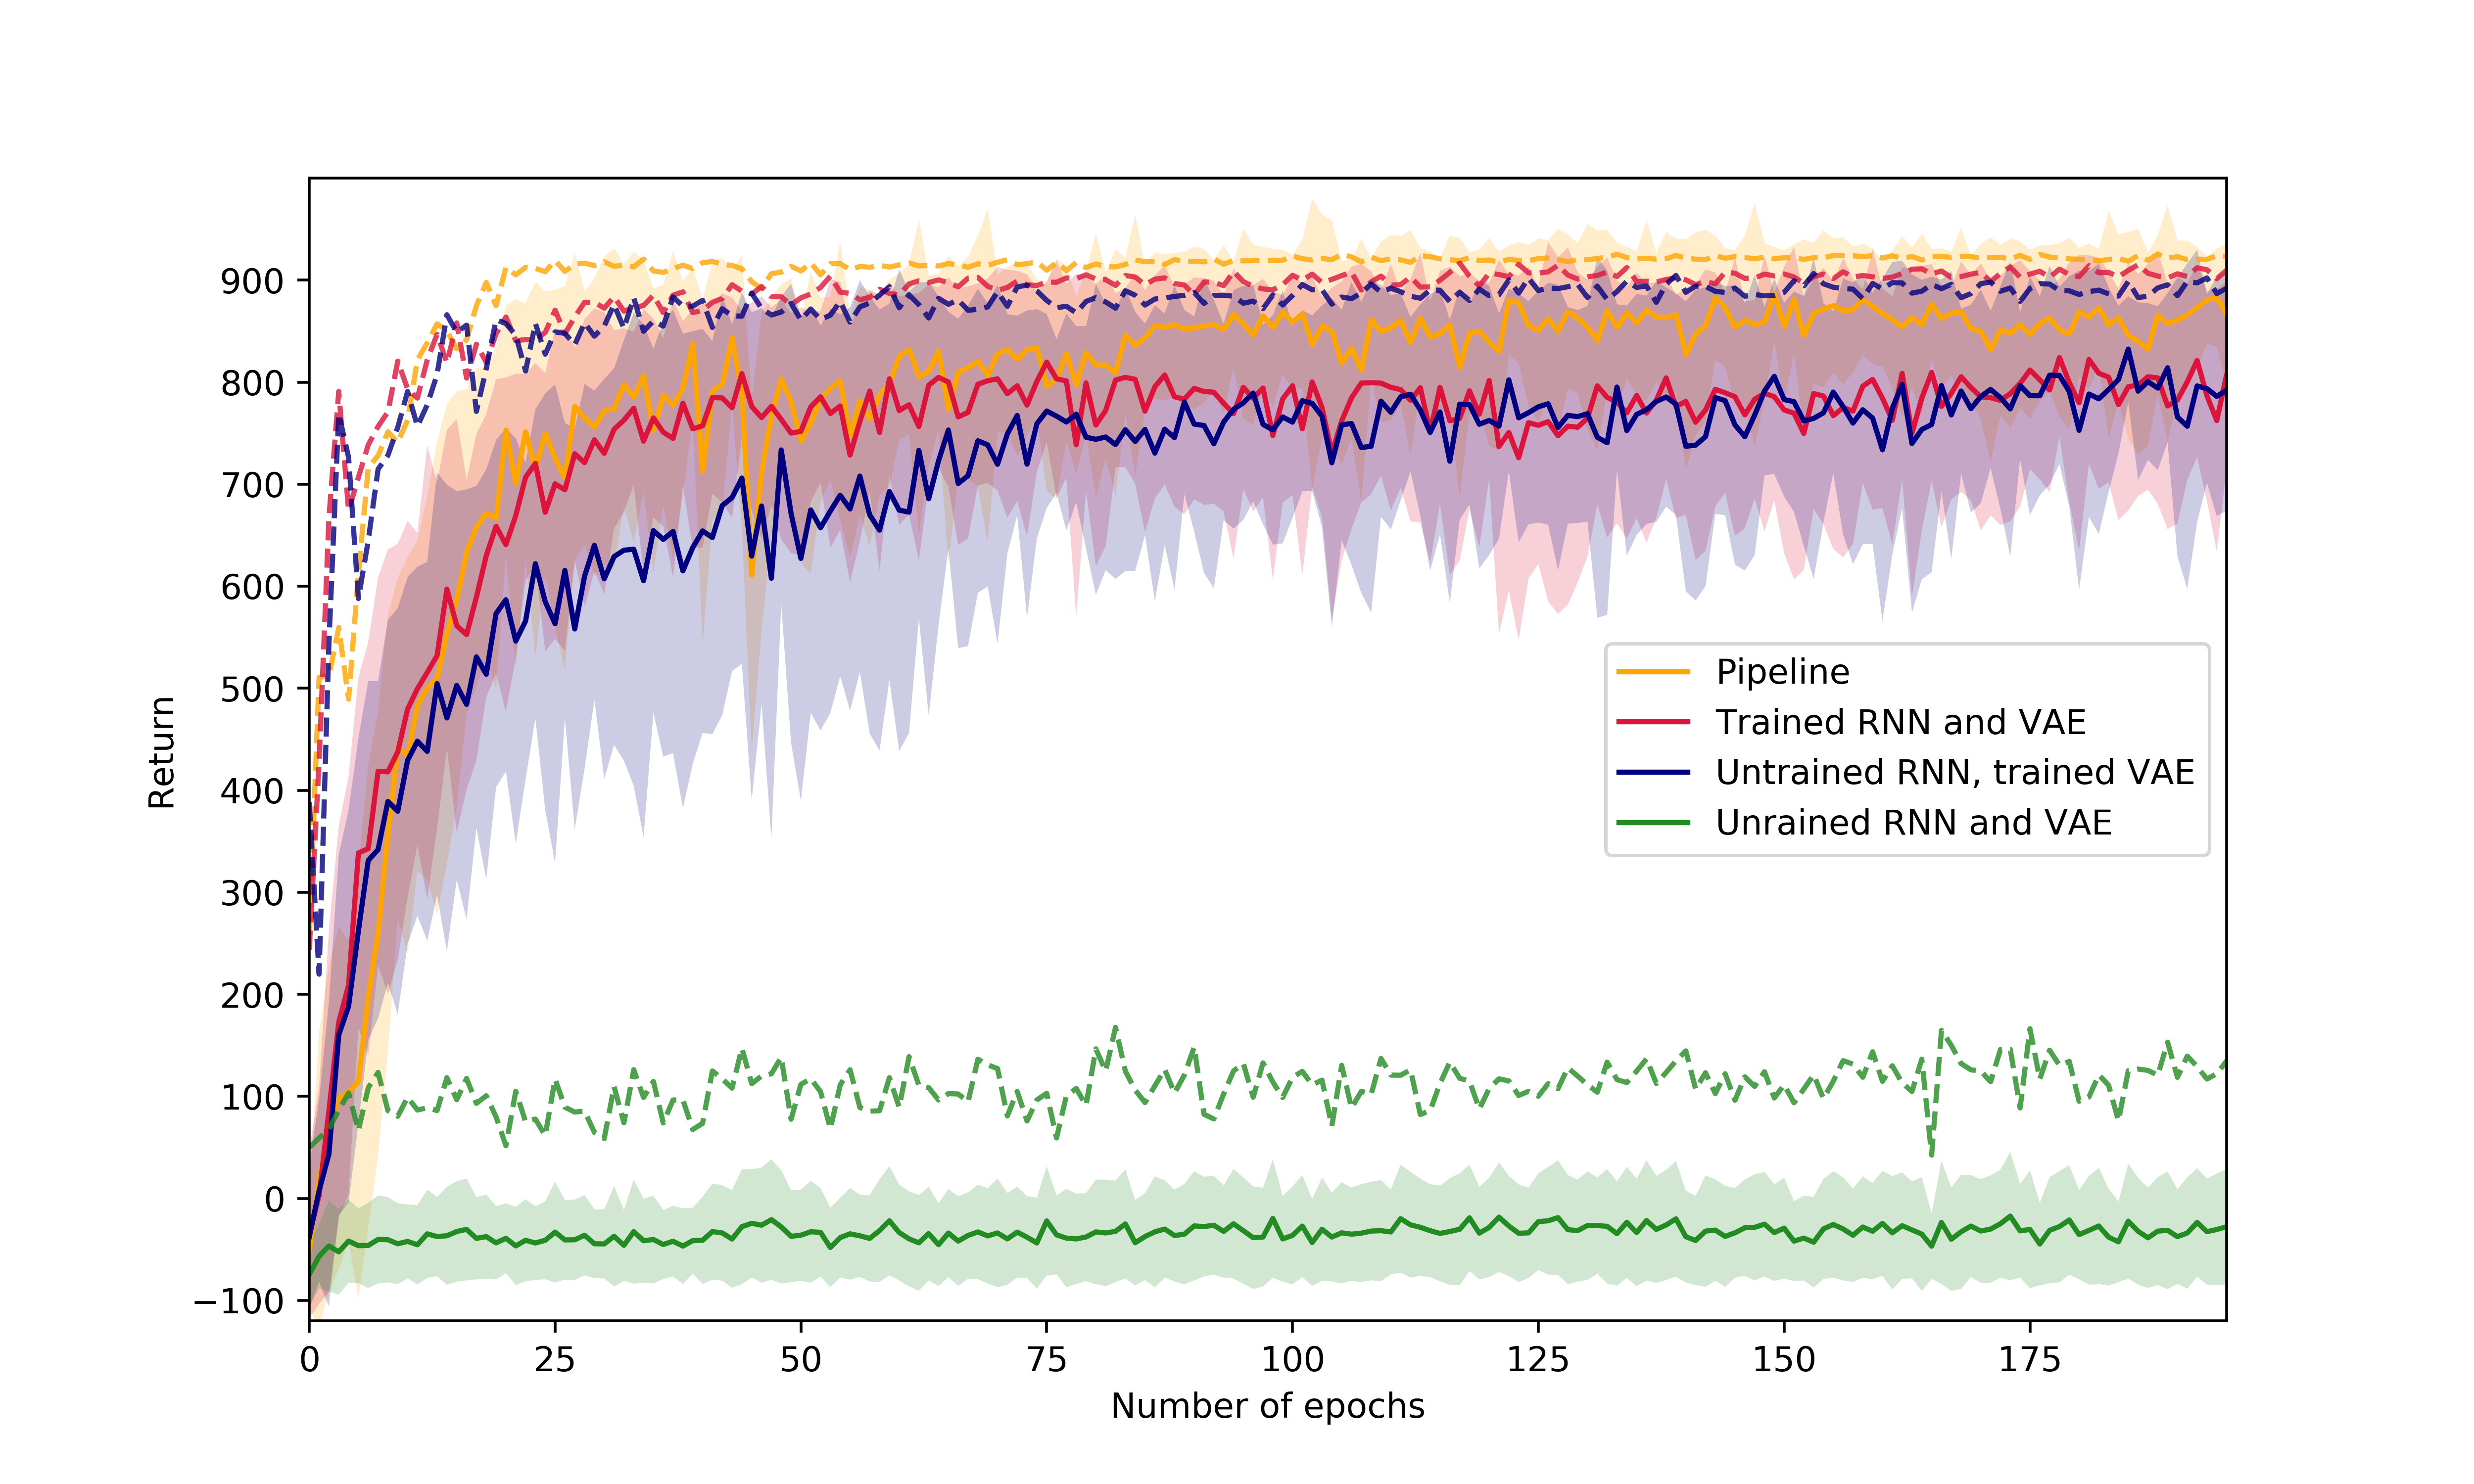
\includegraphics{img/newout.png}
\caption{Learning curves of CMAES. This qualitatively replicates Fig. 4
left from \textcite{NIPS2018_7512}. The number of generations is lower
here, due to computational limitations.}\label{fig:curves}
}
\end{figure}

{\sffamily \small
  \printbibliography[title=References]
}
\end{document}
